\documentclass{scrreprt}
\usepackage[english]{babel}
\usepackage[T1]{fontenc}
\usepackage{lmodern}
\usepackage{blindtext}
\usepackage[utf8]{inputenc}
\usepackage{siunitx} %For unit handling%
\renewcommand{\familydefault}{\sfdefault}
\newcommand{\unit}[1]{\ensuremath{\, \mathrm{#1}}}
\usepackage{amssymb, amsmath, cancel, ulem, graphicx, float, tabularx, multirow, bm}
\usepackage{amsmath}
\usepackage{caption}
\usepackage{subcaption}
\usepackage{tikz}
\newcommand*\circled[1]{\tikz[baseline=(char.base)]{
            \node[shape=circle,draw,inner sep=1pt] (char) {#1};}}
\renewcommand{\phi}{\varphi}

\setcounter{secnumdepth}{5}
\setcounter{tocdepth}{5}

\author{Urs Gerber\\09-921-156 \and Gian-Luca Mateo\\11-113-545}
\date{28th of March 2013}

\title{Forced Oscillation}
\subtitle{Practical course report}

\begin{document}

\maketitle

\tableofcontents
\newpage

\chapter{Experiment: Forced Oscillation}
\section{Introduction}
\subsection{Goal of the experiment}
The goal of this experiment is to determine the resonant frequency and damping coefficient of an osillating system using two different methods: using forced and free oscillations.

\subsection{Theory}
\begin{equation}
J\cdot \ddot{\phi} = \sum_i M_i
\end{equation}
\subsubsection{Free damped oscillation}
\begin{equation}
M_R=-R\dot{\phi}
\end{equation}
\begin{equation}
J\ddot{\phi} + r \dot{\phi} + D \phi = 0
\end{equation}
The solution in case of weak damping is
\begin{equation}
\phi(t) = A e^{-\alpha t} \cos{\left(\omega t - \phi_0\right)}
\end{equation}

\section{Experiment setup and execution}
\subsection{Used materials}
The materials used in this experiment are the following:
\begin{itemize}
\item A hinged metal disc with an indicator at its top connected indirectly to an electric motor using a spring
\item A ring with a printed scale with greater inner radius than the metal disc's diameter
\item An eddy brake
\item An electric engine with 2 analogue regulating knobs for speed regulation
\item A power supply with two outputs, one adjustable at the front at 1-15V / 2A max and the other one at the back fixed at 25V / 0.2A
\item A mechanical stopwatch (0.2s steps)
\item A multimeter (Model FLUKE 73 Multimeter)
\item Six electric wires
\end{itemize}

\subsection{Assembly}

\begin{figure}[H]
	\centering
  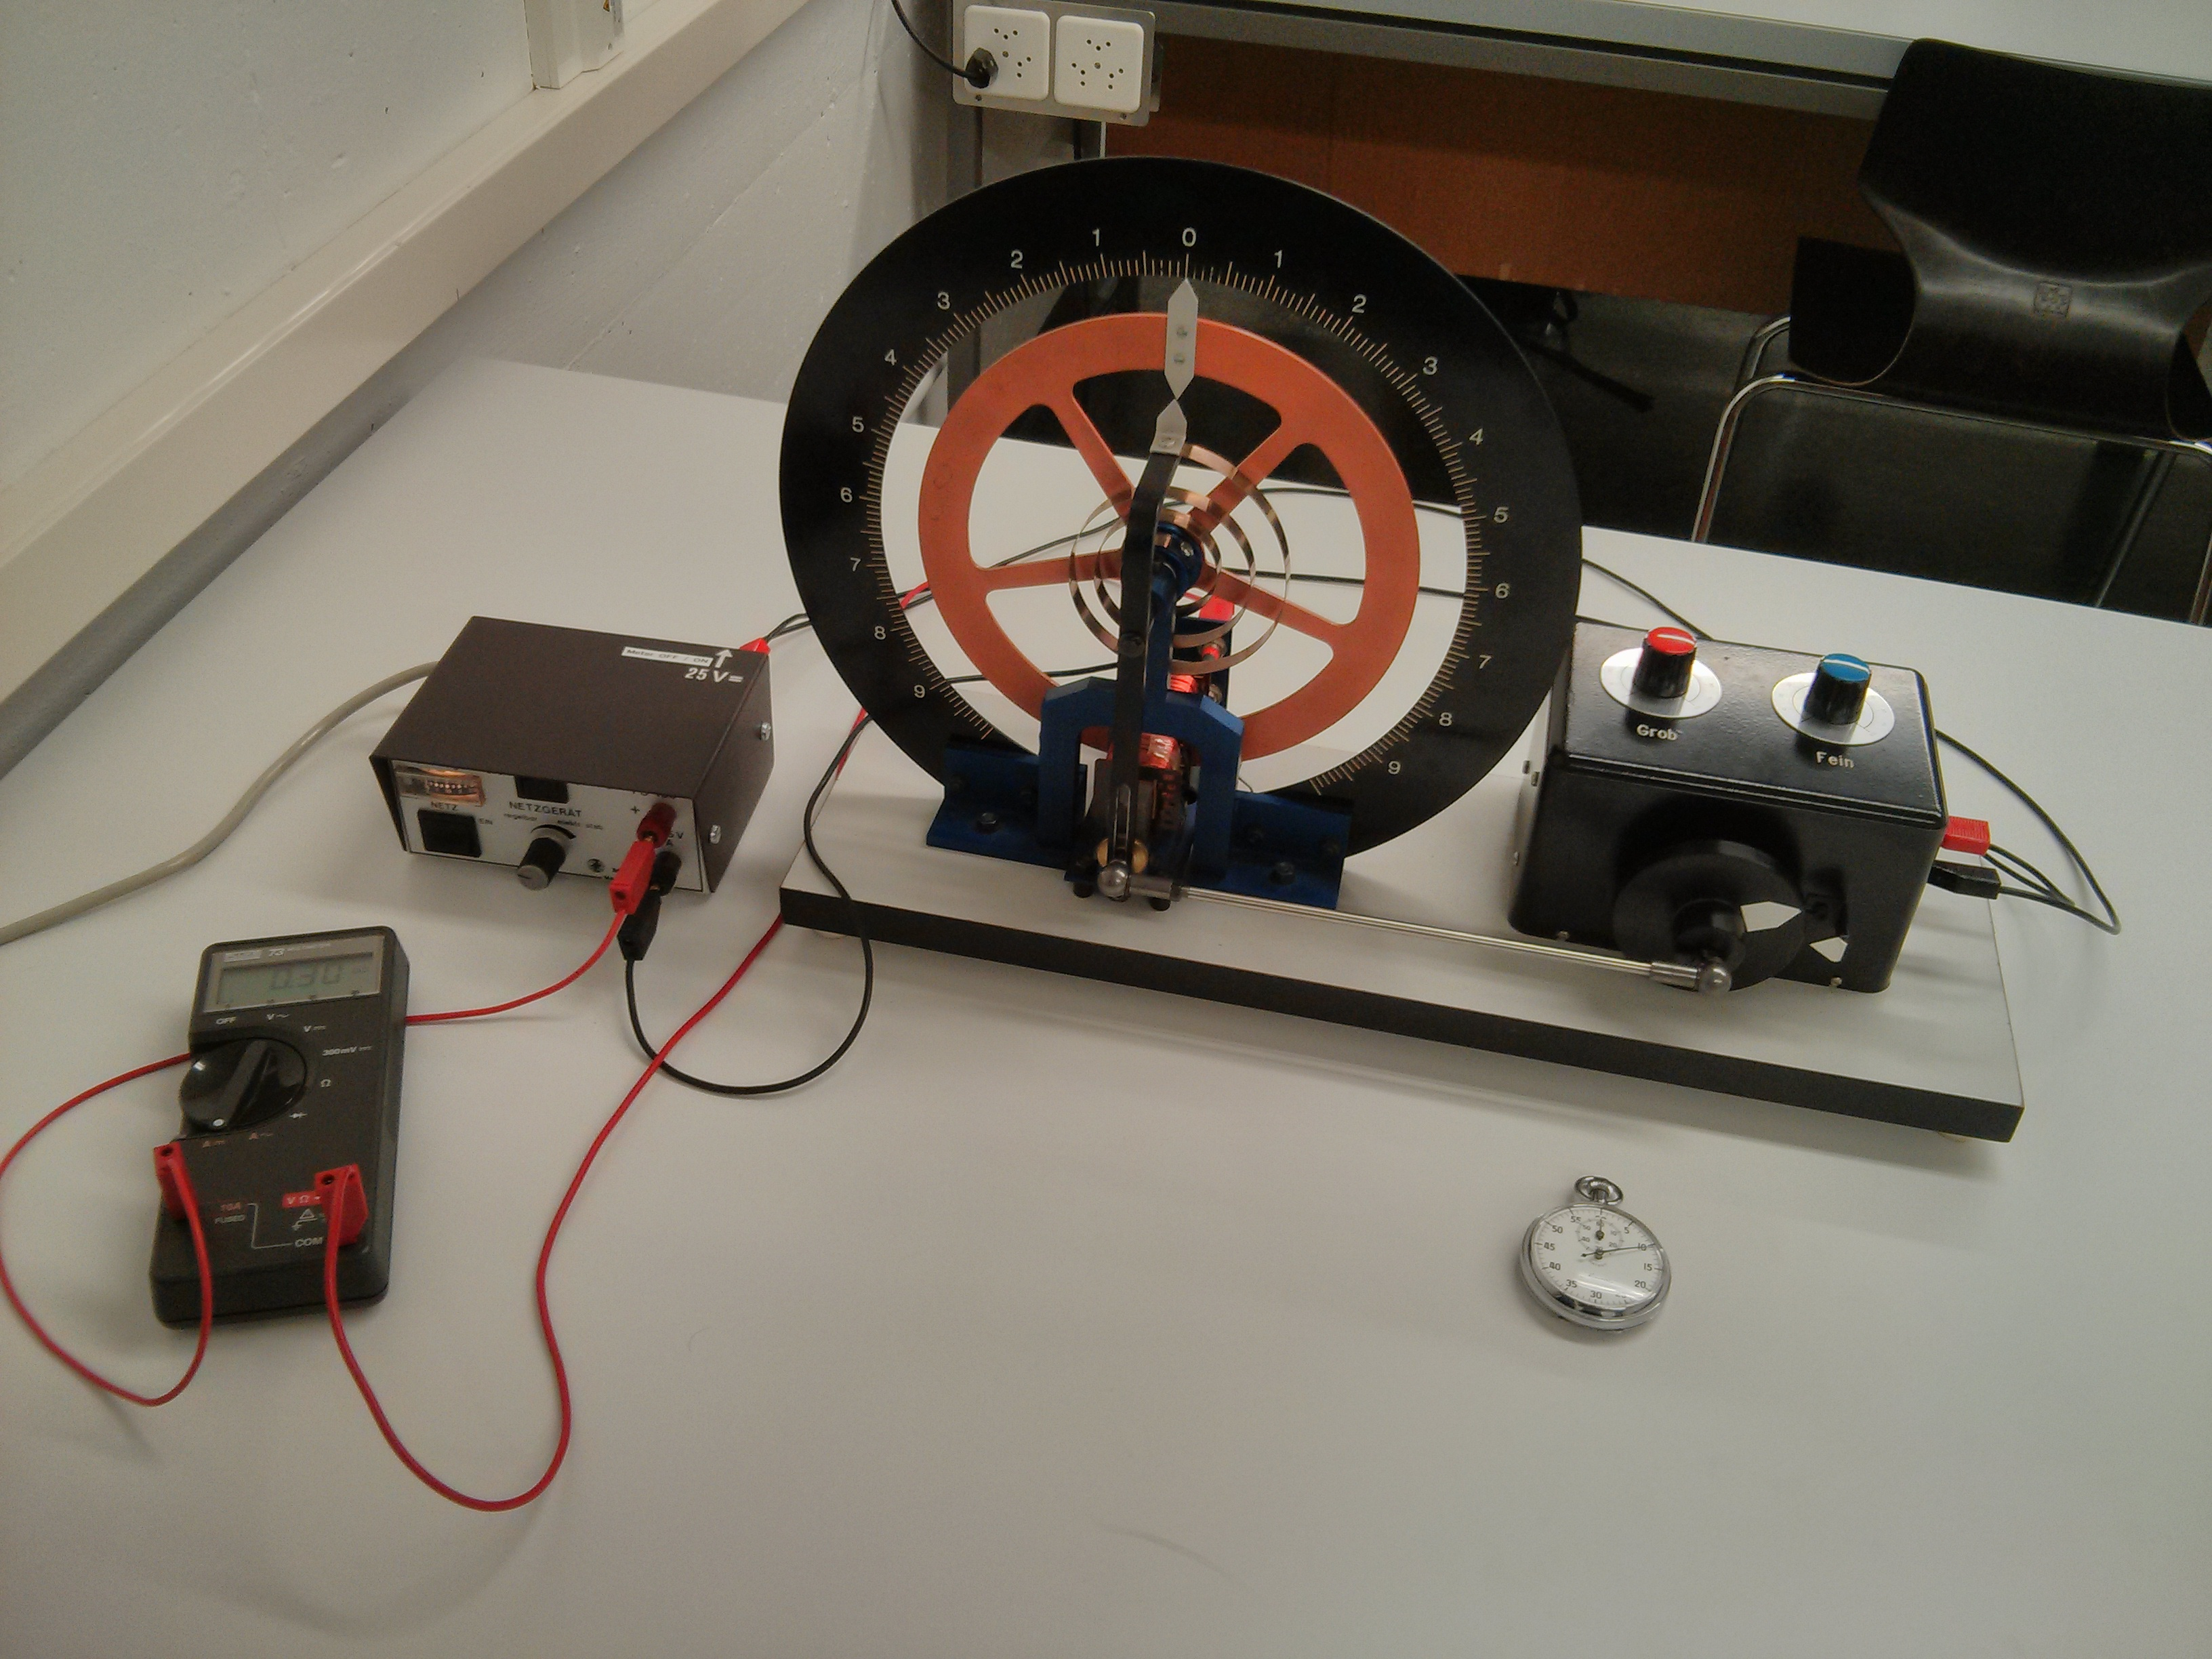
\includegraphics[width=0.9\textwidth]{img/assembly.jpg}
	\caption{The experiment assembly}
	\label{fig:assembly}
\end{figure}

For our measurements, we connect the front output of the power supply to the multimeter and then to the eddy brake and set the multimeter to read the amperage of alternating current. The electric engine is directly connected to the back output of the power supply. The engine is attached to the metal disc using a spring as shown in \ref{fig:assembly}.
\subsubsection{forced oscillation}
For our first measurement series, we set the eddy brake to a certain current and then measured the maximal amplitude of the oscillation at different generator frequencies.
\subsubsection{free oscillation}
For our second mesaurement series we locked the motor and set the eddy brake to the same currents as before plus some others. Then, we moved the disc to an initial deflection and released it, measuring the progression of the maximal amplitudes.

\section{Measurements}
\subsection{forced oscillation}
\begin{figure}[H]
	\centering
  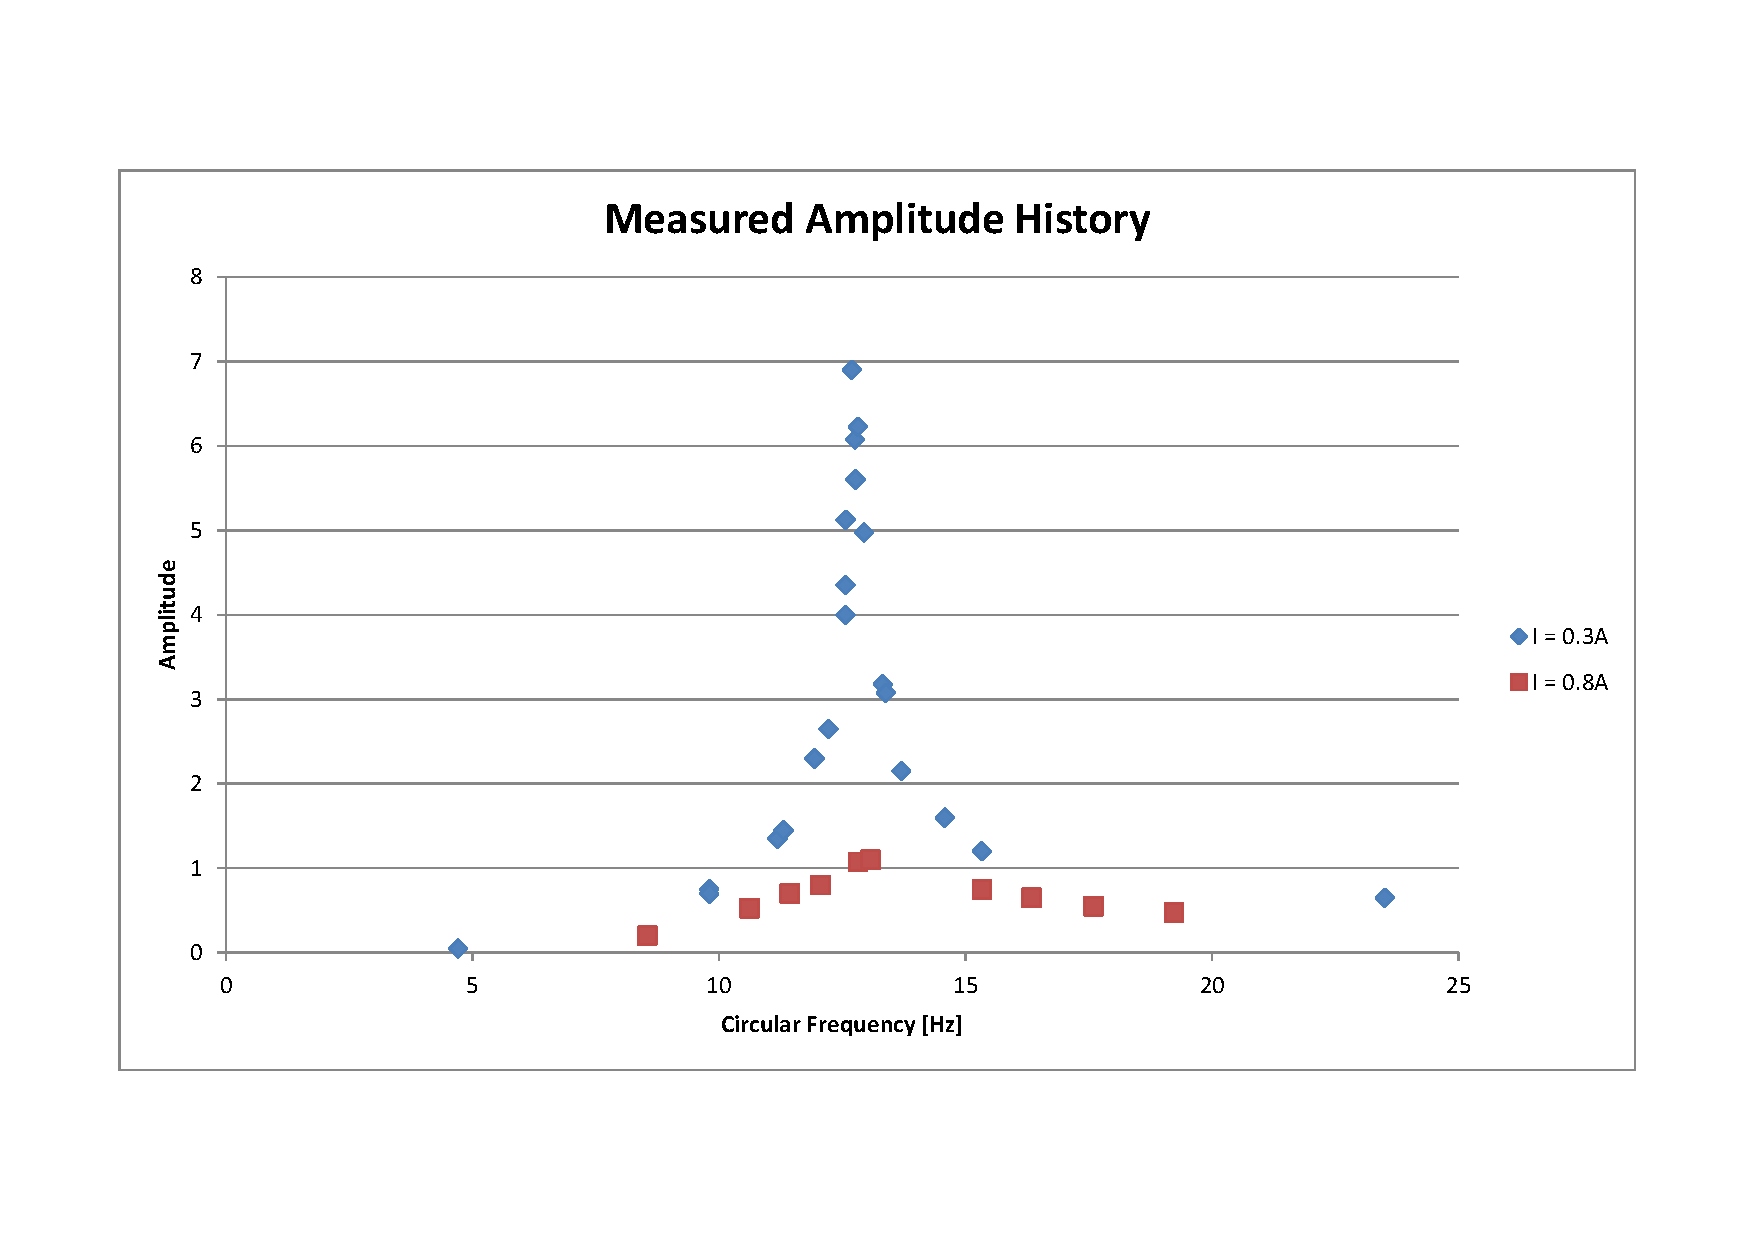
\includegraphics[width=0.9\textwidth]{diag/measurements_amplitudes.pdf}
	\caption{Forced oscillation}
	\label{fig:forcedoscillation}
\end{figure}

\subsection{free oscillation}
\begin{figure}[H]
	\centering
  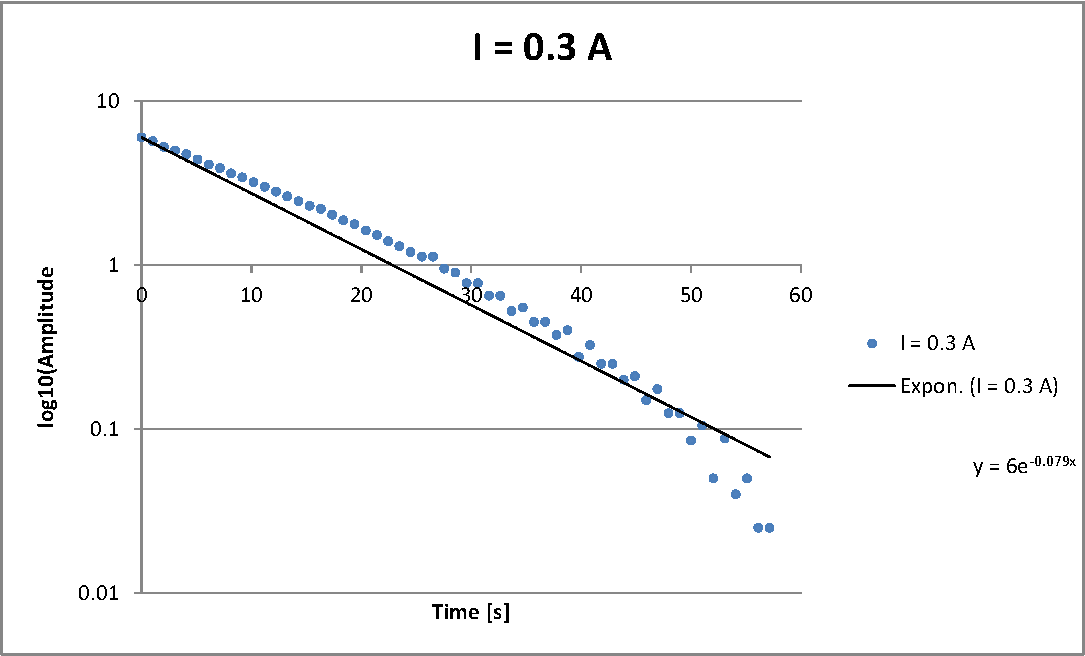
\includegraphics[width=0.9\textwidth]{diag/3A.pdf}
	\caption{Amplitude history over time and exponential approximation}
	\label{fig:0.3A}
\end{figure}

\begin{figure}[H]
	\centering
  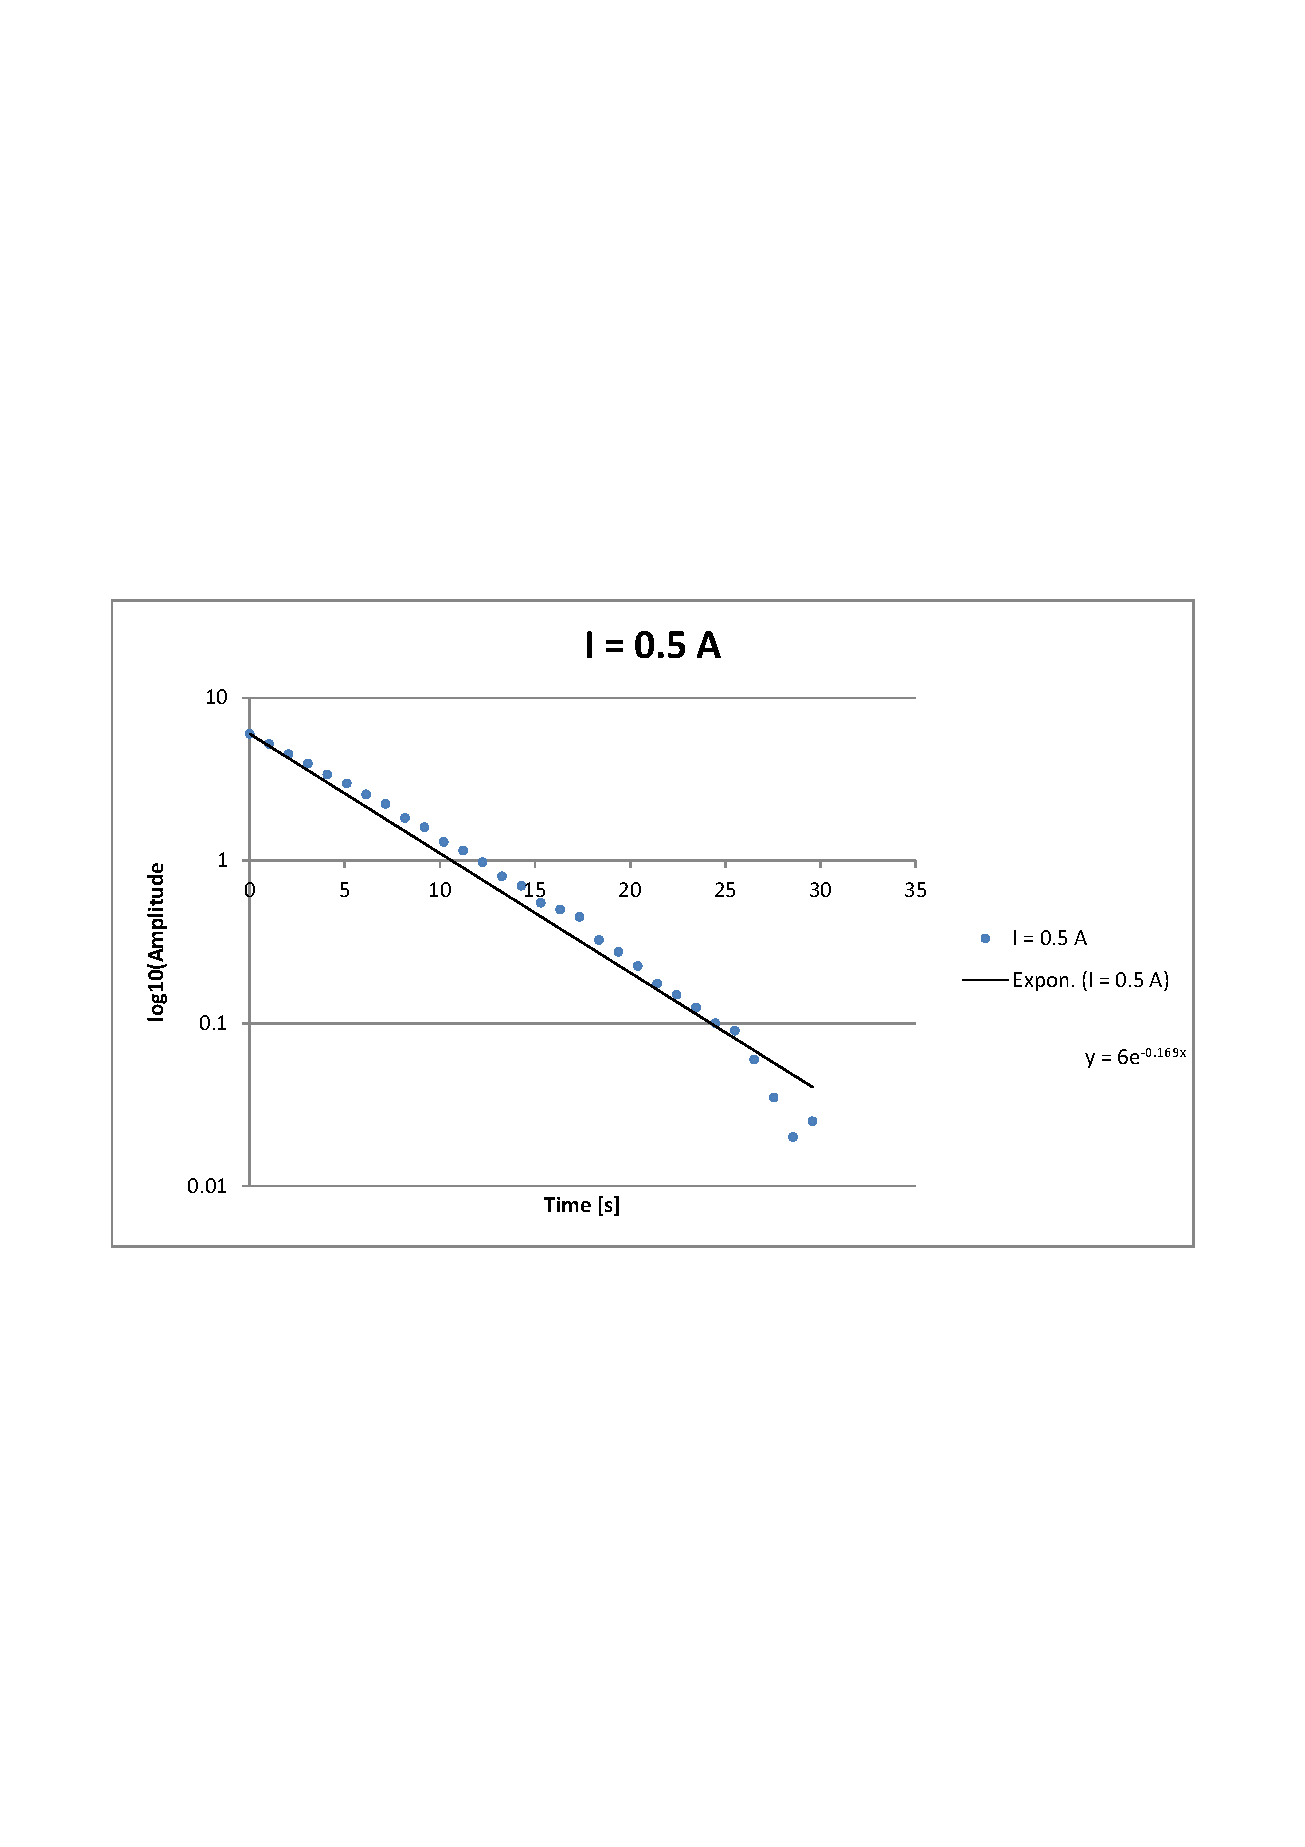
\includegraphics[width=0.9\textwidth]{diag/5A.pdf}
	\caption{Amplitude history over time and exponential approximation}
	\label{fig:0.5A}
\end{figure}

\begin{figure}[H]
	\centering
  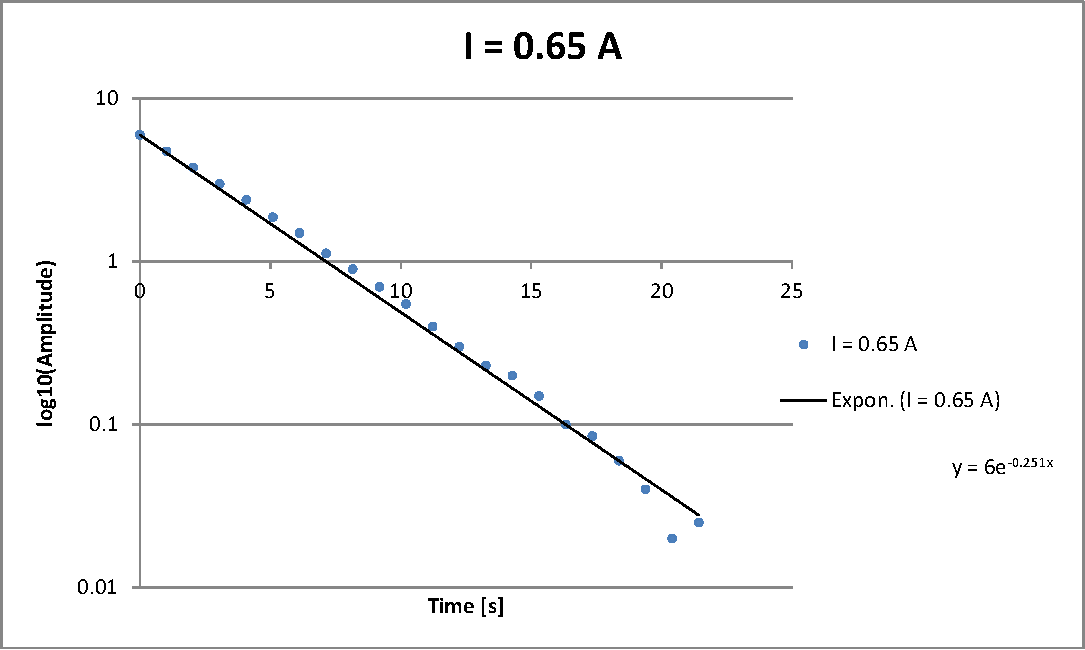
\includegraphics[width=0.9\textwidth]{diag/65A.pdf}
	\caption{Amplitude history over time and exponential approximation}
	\label{fig:0.65A}
\end{figure}

\begin{figure}[H]
	\centering
  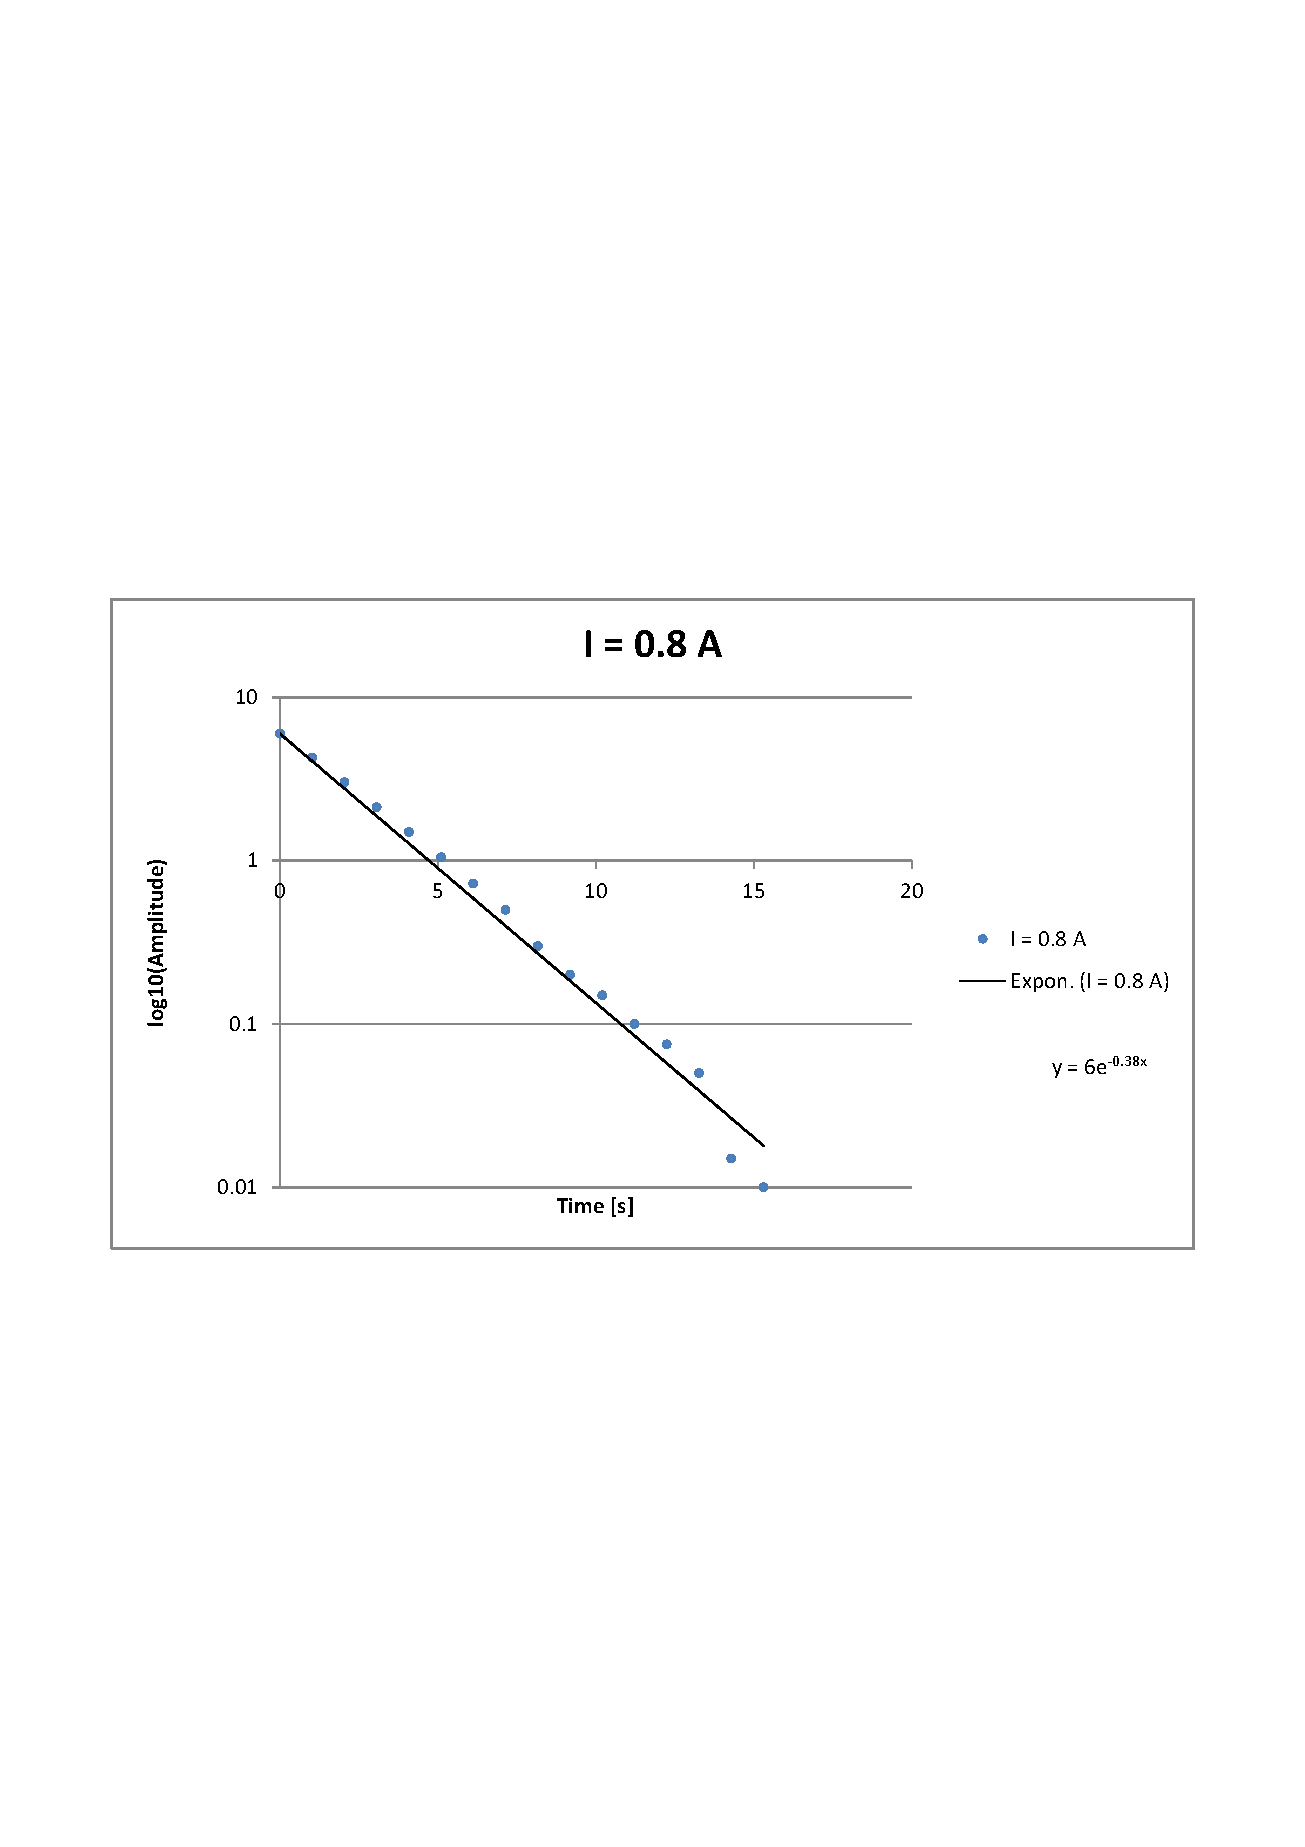
\includegraphics[width=0.9\textwidth]{diag/8A.pdf}
	\caption{Amplitude history over time and exponential approximation}
	\label{fig:0.8A}
\end{figure}


\section{Analysis and Discussion}

\section{Conclusion}


\begin{thebibliography}{9}

\bibitem{physcript13}
  Peter Wurz,
  \emph{Anleitung zum Physikpraktikum}
  FS2013

\end{thebibliography}

\end{document}
